\documentclass[]{beamer}
\usepackage{xmpmulti}
\usepackage{psfrag}
\usepackage{xcolor}
\usepackage{chessboard}
\newcommand{\owner}{\mathcal{O}}
\newcommand{\manager}{\mathcal{M}}

\usepackage{tikz}
\usetikzlibrary{snakes}
\usetikzlibrary{backgrounds} 
\usepackage{pgfmath}


\mode<presentation>
{\usetheme{Boadilla}  % very plain
}

\usepackage{xcolor}

\usepackage{amssymb,amsmath,amsthm}
\usepackage{boxedminipage}

\setbeamercolor{uppercol}{fg=teal,bg=lightgray}%
\setbeamercolor{lowercol}{fg=olive,bg=lightgray!50}%

\newcommand{\curr}{\mathtt{current}}
\newcommand{\mos}{\mathtt{m}}
\newcommand{\move}{\mathtt{lmove}}
\newcommand{\nmove}{\mathtt{nmove}}

\title[]{Binary Search}

\author{Giuseppe Persiano}

\institute[UNISA]{%
Universit\`a di Salerno\\ \qquad \\
}

\date[Ottobre 2020]{Ottobre, 2020}

\begin{document}

{
\begin{frame}
  \titlepage
\end{frame}

\begin{frame}
\frametitle{Cercare un elemento in una Lista}

Impieghiamo tempo $O(N)$

Se la lista \`e {\bf ordinata} riusciamo a farlo in tempo $O(\log N)$
\end{frame}

\begin{frame}
\begin{block}{\bf Ricerca binaria}
\begin{enumerate}[<+->]
\color{blue}
\item Abbiamo una lista ordinata $\color{magenta} A$ di $\color{magenta} N$ elementi: $\color{magenta} A[0],\ldots,A[N-1]$
\item\color{blue} Vogliamo cercare l'elemento $\color{magenta} x$
    \begin{itemize}
        \color{blue}
        \item trovare $\color{magenta} i$ tale che $A\color{magenta} [i]=x$
            \begin{itemize}
            \color{blue}
            \item Se $A\color{magenta} =[3,5,8,9,14]$ e $\color{magenta} x=8$ allora $\color{magenta} i=2$
            \end{itemize}
        \item trovare $\color{magenta} i$ tale che se inseriamo $\color{magenta} x$ alla posizione $\color{magenta} i$, $\color{magenta} A$ resta ordinato.
            \begin{itemize}
            \color{blue}
            \item Se $\color{magenta} A=[3,5,8,9,14]$ e $\color{magenta} x=4$ allora $\color{magenta} i=1$
            \item {\tt A.insert(1,4)=[3,{\color{green} 4},5,8,9,14]}
            \end{itemize}
    \end{itemize}
\item All'inizio so che $\color{magenta} l=0\leq i\leq h=N-1$
\item Se $\color{magenta} l>h$, return $\color{magenta} l$
\item Calcolo indice centrale $\color{magenta} m=(h+l)//2$
\item Tre casi sono possibili
    \begin{itemize}
            \color{blue}
        \item $\color{magenta} A[m]=x$. Return $\color{magenta} i=m$
        \item $\color{magenta} A[m]<x$. Allora so che $\color{magenta} l\leq i\leq h=m-1$
        \item $\color{magenta} A[m]>x$. Allora so che $\color{magenta} l=m+1\leq i\leq h$
    \end{itemize}
\item Torna al passo $4$

\end{enumerate}
\end{block}
\end{frame}

\color{black}
\begin{frame}
\begin{tikzpicture}
[
cs/.style={rectangle,draw=green!50,fill=black!10,thick,minimum height=7mm,minimum width=70mm},
stack/.style={rectangle,draw=black!50,fill=black!20,thick,minimum height=7mm,minimum width=70mm},
nm/.style={rectangle,draw=black!50,fill=green!20,thick,minimum size=7mm},
]
\only<1>{\node (0,0) (array) {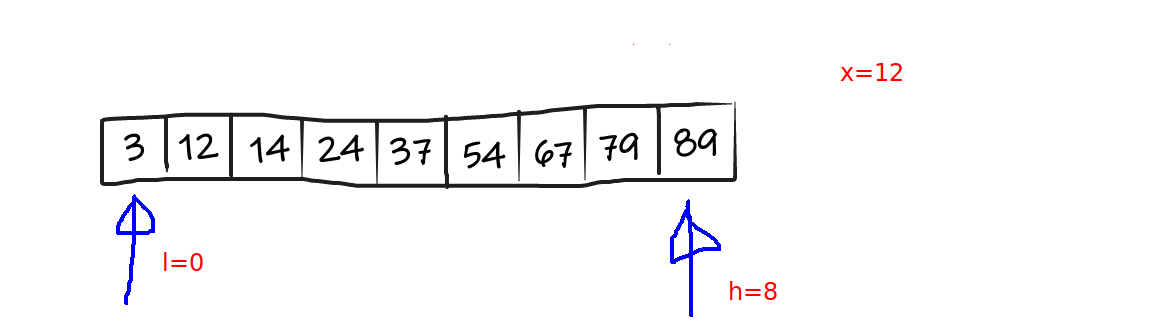
\includegraphics[width=5in]{02.png}};
         \node [below=3cm] at (array) {\color{blue} Cerchiamo $x$ tra l'indice $l=0$ e l'indice $h=8$};
}
\only<2>{\node (0,0) (array) {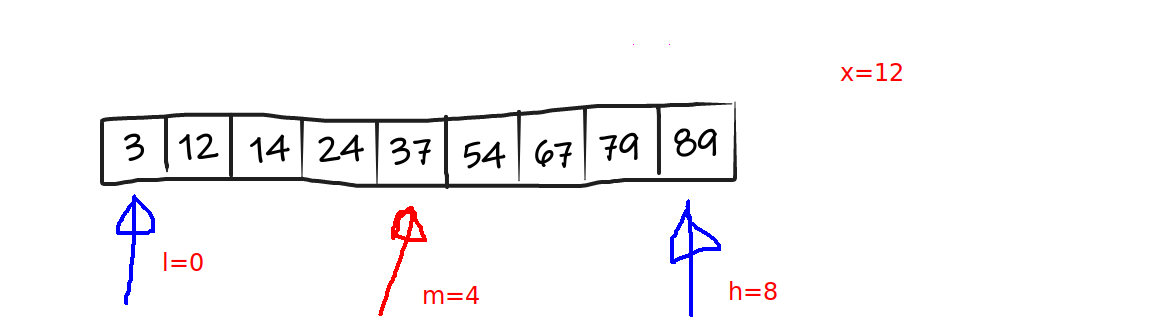
\includegraphics[width=5in]{03.png}};
         \node [below=3cm] at (array) {\color{blue} Cerchiamo $x$ tra l'indice $l=0$ e l'indice $h=8$};
         \node [below=4cm,anchor=west] at (array) {\color{blue} $m=4$ e $A[m]>x$};
}
\only<3>{\node (0,0) (array) {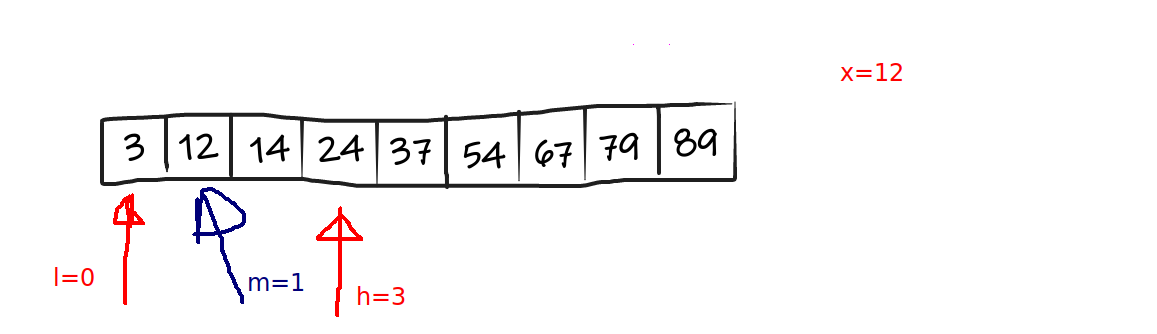
\includegraphics[width=5in]{04.png}};
         \node [below=3cm] at (array) {\color{blue} Cerchiamo $x$ tra l'indice $l=0$ e l'indice $h=3$};
         \node [below=4cm,anchor=west] at (array) {\color{blue} $m=1$ e $A[m]=x$};
        }
\end{tikzpicture}
\end{frame}

\begin{frame}
\frametitle{Complessit\`a di Ricerca Binaria}

\begin{itemize}[<+->]
\item Ad ogni passo, l'intervallo si dimezza
\vskip 1cm
\item Ci fermiamo quando l'intervallo ha solo $l$
\vskip 1cm
\item Al massimo $O(\log N)$ passi
\end{itemize}
\end{frame}

\end{document}

